\documentclass[10pt,journal]{IEEEtran}
\usepackage[spanish]{babel}
\addto\captionsspanish{\renewcommand{\tablename}{Tabla}}
\usepackage[T1]{fontenc}
\usepackage{amsmath}
\usepackage{amssymb}
\usepackage{float}
\usepackage{graphicx}
\usepackage{booktabs}
\usepackage{placeins}
\usepackage{xcolor}
\usepackage{listings}

\lstdefinestyle{pythonstyle}{
  language=Python,
  basicstyle=\ttfamily\small,
  keywordstyle=\color{blue!60!black}\bfseries,
  stringstyle=\color{red!50!brown},
  commentstyle=\color{gray}\itshape,
  numbers=none,
  breaklines=true,
  showstringspaces=false,
  frame=single,
  framesep=3pt,
  xleftmargin=3pt,
  xrightmargin=3pt,
  columns=flexible,
}
\lstset{style=pythonstyle}
\usepackage[pdfauthor={Jheison Martinez Bolivar},pdftitle={Aprendizaje No Supervisado sobre Objetos Celestes del SDSS DR17},colorlinks,linkcolor=blue,citecolor=green,urlcolor=cyan]{hyperref}

% ---------------------------------------------------------------
% Enlace al cuaderno. Reemplazar por la URL definitiva de Colab.
\newcommand{\enlacenb}{https://colab.research.google.com/drive/1vBsjBbquzO43cMjuuwck8IQBVHYOaMvX?usp=sharing}
% ---------------------------------------------------------------

\begin{document}

  \title{Aprendizaje No Supervisado sobre Objetos Celestes del {SDSS} {DR17}:\\
    An\'alisis de Componentes Principales, K-medias y Mezclas Gaussianas}

  \author{
    Jheison Martinez Bolivar\\
    \textit{Maestr\'ia en Inteligencia Artificial}\\
    \textit{Universidad de La Salle, Bogot\'a, Colombia}\\
    \texttt{jhmartinez07@unisalle.edu.co}
  }
  \maketitle
  \markboth{Universidad de La Salle --- Aprendizaje de M\'aquina. Septiembre 2026}{}

  \begin{abstract}
    Este trabajo aplica aprendizaje no supervisado sobre 100\,000 objetos celestes del \emph{Sloan Digital Sky Survey} Data Release 17, con el objetivo de determinar cu\'anto de la clasificaci\'on espectrosc\'opica oficial (\texttt{GALAXY}, \texttt{STAR}, \texttt{QSO}) puede recuperarse \'unicamente a partir de las cinco magnitudes fotom\'etricas \emph{ugriz}. La etiqueta se apart\'o desde el inicio y se us\'o solo como vara de medici\'on externa. Una auditor\'ia de las 18 columnas mediante informaci\'on mutua con l\'inea base por permutaci\'on llev\'o a excluir \texttt{redshift} por fuga de informaci\'on ---el corrimiento al rojo y el tipo espectral se determinan de forma conjunta e inseparable en el mismo ajuste de plantillas--- y a excluir \texttt{plate}, \texttt{MJD} y \texttt{run\_ID} por corresponder a la log\'istica de observaci\'on del propio sondeo. Sobre las cinco bandas se aplic\'o PCA: dos componentes concentran el 97.4\,\% de la varianza, pero el componente dominante (PC1, 85.6\,\% de varianza) es de los menos informativos sobre el tipo (0.068 nats, cuarto de cinco componentes), mientras que PC2 (11.8\,\% de varianza) es el m\'as informativo (0.294 nats). Esa disociaci\'on domina los resultados: K-medias parte los datos exclusivamente a lo largo de PC1 y alcanza $AMI=0.0473$, mientras que una mezcla gaussiana con covarianza \texttt{full} sobre tres componentes alcanza $AMI=0.2434$. La comparaci\'on de \texttt{covariance\_type} muestra una progresi\'on mon\'otona (\texttt{spherical} 0.0490, \texttt{tied} 0.0750, \texttt{diag} 0.1441, \texttt{full} 0.2434) que no se explica con una sola libertad geom\'etrica. El mejor modelo asigna el 85.4\,\% de los objetos con m\'as del 90\,\% de certeza pese a un AMI de 0.24: alta confianza y baja correspondencia con la verdad conviven sin contradicci\'on. El cuaderno con la implementaci\'on completa est\'a disponible en Google Colab: \url{\enlacenb}.
  \end{abstract}

  \section{Introducci\'on}

  \IEEEPARstart{E}{l} \emph{Sloan Digital Sky Survey} (SDSS) observa el cielo de dos maneras que cuestan cosas muy distintas. La primera es la \textbf{fotometr\'ia}: una c\'amara mide cu\'anta luz llega de un objeto a trav\'es de cinco filtros de colores ---$u$ (ultravioleta), $g$ (verde-azul), $r$ (rojo), $i$ (infrarrojo cercano) y $z$ (infrarrojo)--- y produce cinco n\'umeros por objeto \cite{fukugita1996}. Es barata y se aplica a todo lo que entra en el campo de visi\'on. La segunda es la \textbf{espectroscop\'ia}: se dirige una fibra \'optica a un objeto concreto y se descompone su luz en un espectro completo, del cual el \emph{pipeline} del sondeo deriva tanto su tipo (\texttt{GALAXY}, \texttt{STAR}, \texttt{QSO}) como su corrimiento al rojo \cite{bolton2012}. Es cara, lenta y limitada a los objetos que se decida apuntar.

  Conviene precisar el significado f\'isico de las cinco magnitudes, porque no se comportan como una medici\'on ordinaria: la magnitud astron\'omica es \emph{logar\'itmica e invertida}. La escala moderna fija la raz\'on de brillo entre dos magnitudes consecutivas en $100^{1/5} \approx 2.512$ \cite{pogson1856}, y hereda de los cat\'alogos cl\'asicos el orden invertido, de modo que un n\'umero m\'as peque\~no corresponde a un objeto m\'as brillante. Su valor absoluto mezcla dos cosas distintas ---cu\'anta luz emite el objeto y qu\'e tan lejos est\'a---, mientras que la \emph{diferencia} entre dos bandas ($u-g$, $g-r$, \dots), llamada \emph{color}, describe la forma del espectro y es en principio independiente de la distancia. Esta distinci\'on entre brillo y color reaparecer\'a como el eje central de todo el an\'alisis.

  El problema que aborda este trabajo es directo: \textbf{si solo se tuvieran las cinco magnitudes fotom\'etricas, sin espectro y sin etiqueta, \textquestiondown{}cu\'anto de la clasificaci\'on oficial se podr\'ia reconstruir?} La pregunta no es acad\'emica: los sondeos fotom\'etricos producen \'ordenes de magnitud m\'as objetos de los que alcanza a cubrir la espectroscop\'ia, de manera que cualquier estructura recuperable desde la fotometr\'ia sola tiene valor pr\'actico para priorizar qu\'e observar.

  Se aplican tres t\'ecnicas no supervisadas de naturaleza complementaria: \textbf{An\'alisis de Componentes Principales} (PCA) como reducci\'on de dimensionalidad \cite{hotelling1933,jolliffe2016}, \textbf{K-medias} como particionamiento geom\'etrico \cite{macqueen1967,lloyd1982} y \textbf{mezclas gaussianas} (GMM) como modelo probabil\'istico generativo \cite{dempster1977,mclachlan2000}. La etiqueta \texttt{class} se apart\'o antes de tocar los datos y no particip\'o en ning\'un entrenamiento; se reserv\'o \'unicamente como \emph{vara de medici\'on externa} mediante informaci\'on mutua ajustada \cite{vinh2010}. El objetivo no es maximizar una m\'etrica, sino entender \emph{qu\'e} estructura encuentra cada algoritmo y \emph{por qu\'e} esa estructura coincide o no con la clasificaci\'on f\'isica.

  \section{Datos y Preprocesamiento}

  \subsection{Conjunto de Datos}

  Se emple\'o el cat\'alogo \emph{Stellar Classification Dataset SDSS17} \cite{kaggle_sdss_dataset}, una extracci\'on de 100\,000 objetos y 18 columnas del Data Release 17 del SDSS \cite{abdurrouf2022}. La variable \texttt{class} distribuye los objetos en \texttt{GALAXY} (59\,445 objetos, 59.4\,\%), \texttt{STAR} (21\,594, 21.6\,\%) y \texttt{QSO} (18\,961, 19.0\,\%). No hay valores nulos.

  Las 18 columnas provienen de tres or\'igenes distintos, distinci\'on que resulta central para la selecci\'on de variables: siete son fotom\'etricas (las cinco bandas \emph{ugriz} m\'as las coordenadas celestes \texttt{alpha} y \texttt{delta}), seis son espectrosc\'opicas (\texttt{spec\_obj\_ID}, \texttt{class}, \texttt{redshift}, \texttt{plate}, \texttt{MJD}, \texttt{fiber\_ID}) y el resto son identificadores de la operaci\'on del telescopio (\texttt{obj\_ID}, \texttt{run\_ID}, \texttt{rerun\_ID}, \texttt{cam\_col}, \texttt{field\_ID}). Es importante consignar una limitaci\'on de partida: \textbf{el conjunto de datos no incluye un diccionario de columnas}, de modo que esta separaci\'on se infiri\'o de los nombres de las variables y del funcionamiento documentado del SDSS \cite{sdss_dr17_columns}. Es una suposici\'on apoyada en el dominio, no una verificaci\'on en la fuente.

  \subsection{An\'alisis Exploratorio}

  La auditor\'ia de cardinalidad revel\'o dos casos degenerados: \texttt{rerun\_ID} es constante (un \'unico valor en las 100\,000 filas, por lo que no puede informar nada) y \texttt{spec\_obj\_ID} toma un valor distinto por fila (es una clave primaria, no una medici\'on).

  Las bandas presentan un artefacto de instrumentaci\'on: el resumen estad\'istico muestra m\'inimos de $-9999$ en $u$, $g$ y $z$, con desviaciones est\'andar infladas a $\sim$31.7 frente a $\sim$1.8 en $r$ e $i$. Ese valor es un c\'odigo centinela de medici\'on fallida, no una magnitud. Afecta a \textbf{una sola fila} de las 100\,000, que se elimin\'o; el an\'alisis contin\'ua sobre 99\,999 objetos.

  La Figura~\ref{fig:correlacion} muestra la correlaci\'on de Pearson entre todas las columnas num\'ericas. Las cinco bandas forman un bloque fuertemente correlacionado entre s\'i (nueve de los diez pares superan $r=0.6$; el m\'aximo es $r=0.972$ entre $i$ y $z$, y el m\'inimo $r=0.546$ entre $u$ y $z$, los dos extremos del rango de longitudes de onda): un objeto brillante lo es en todas las bandas a la vez. Esta redundancia es exactamente la condici\'on que hace apropiado un PCA. Las coordenadas celestes y los identificadores, en cambio, no correlacionan de forma apreciable con las bandas.

  \begin{figure*}[t]
    \centering
    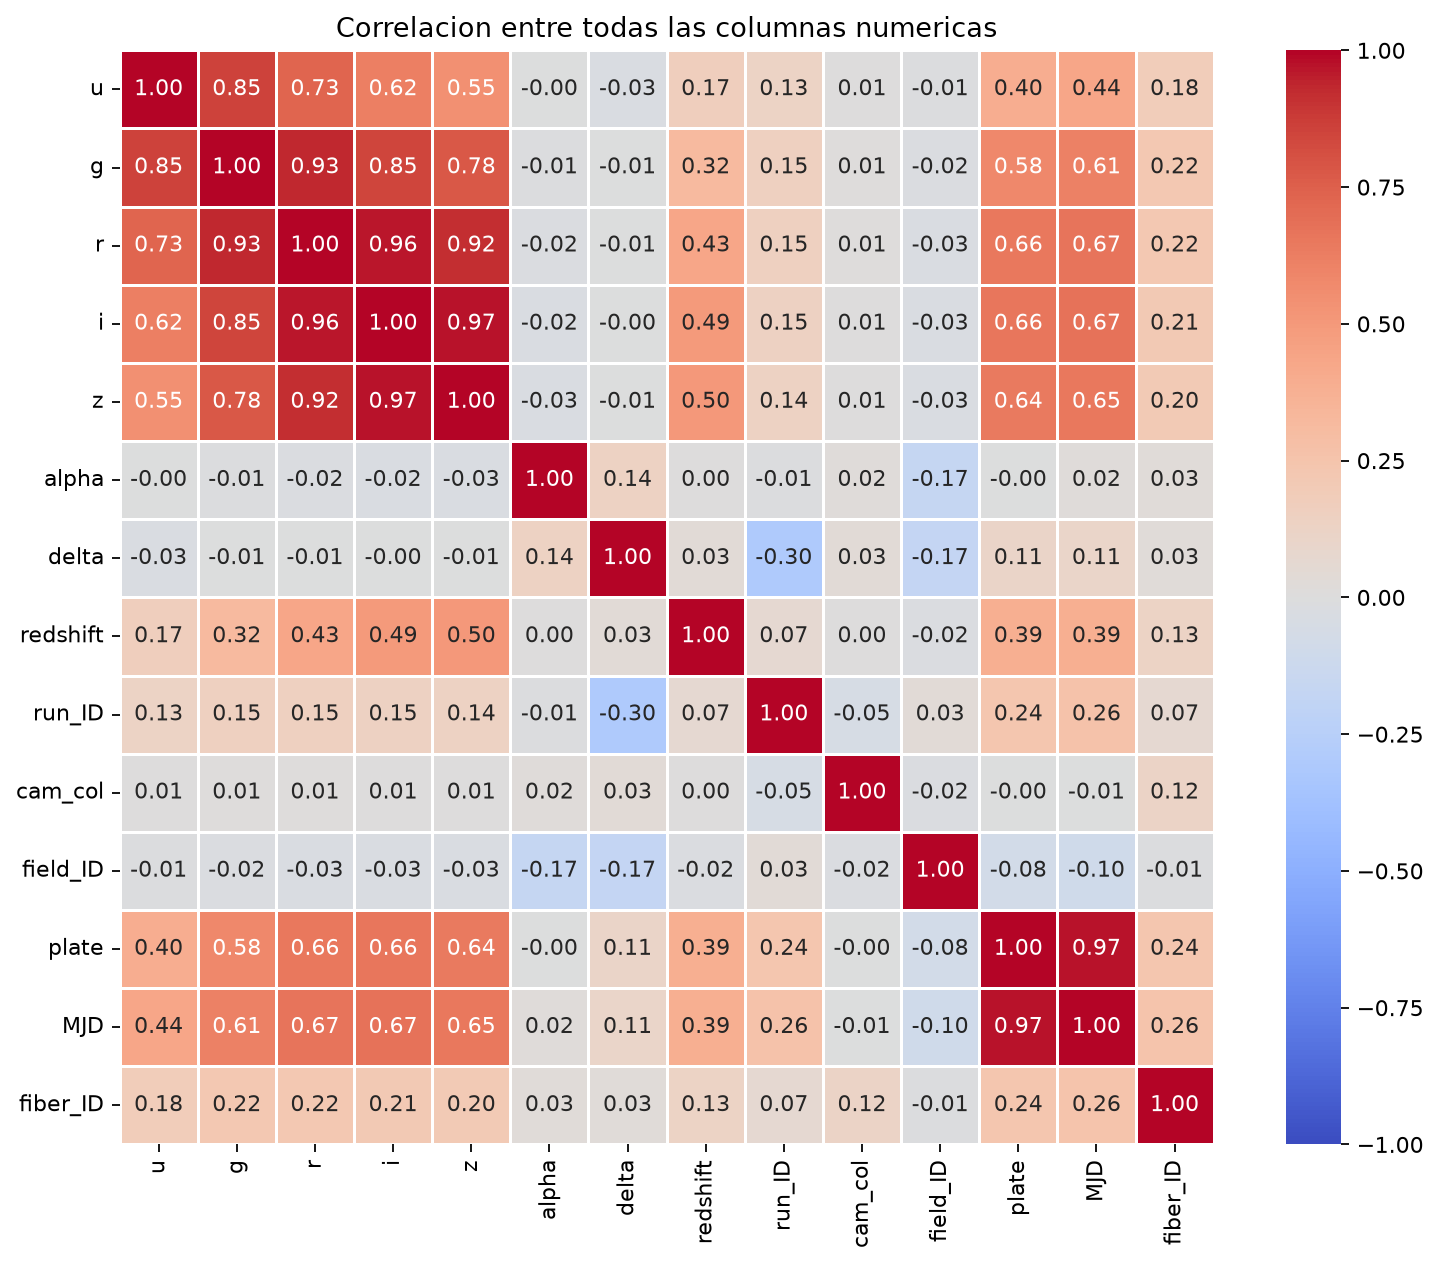
\includegraphics[width=0.72\linewidth]{assets/images/fig_correlacion.png}
    \caption{Correlaci\'on de Pearson entre las columnas num\'ericas. El bloque de las cinco bandas \emph{ugriz} concentra la redundancia que justifica el PCA.}
    \label{fig:correlacion}
  \end{figure*}

  \subsection{Auditor\'ia de Variables y Fuga de Informaci\'on}
  \label{sec:auditoria}

  Descartar variables por intuici\'on es un riesgo, as\'i que la selecci\'on se hizo midiendo. Se calcul\'o la \textbf{informaci\'on mutua} entre cada columna candidata y la etiqueta \cite{cover2006}, con el estimador por vecinos m\'as cercanos de \texttt{scikit-learn} \cite{ross2014,pedregosa2011}. La informaci\'on mutua tiene una trampa conocida: una variable con muchos valores distintos obtiene una puntuaci\'on alta incluso cuando no guarda ninguna relaci\'on real con la etiqueta, simplemente porque cada valor identifica a pocas filas. Es el mismo sesgo por el que la informaci\'on mutua entre particiones debe corregirse por el acuerdo esperado al azar \cite{vinh2010}. Para acotarla se calcul\'o adem\'as una \textbf{l\'inea base por permutaci\'on}: se baraj\'o la etiqueta al azar tres veces y se promedi\'o la informaci\'on mutua obtenida contra esa etiqueta sin sentido. La diferencia entre la medici\'on real y esa l\'inea base es la se\~nal atribuible. Tres r\'eplicas son pocas para estimar esa l\'inea con precisi\'on, pero basta para lo que se decide con ella. La correcci\'on que aporta es a lo sumo de 0.069 nats (el caso de \texttt{plate}, la columna de mayor cardinalidad), entre dos y cuatro veces menor que los excesos sobre los que se sustentan las exclusiones; para el resto de columnas la desproporci\'on es mucho mayor (\texttt{run\_ID}: 0.0044 de l\'inea base frente a 0.1432 de exceso). La l\'inea tendr\'ia que estar muy mal estimada para alterar el orden. La Figura~\ref{fig:mi} presenta el resultado, con la entrop\'ia de la etiqueta (0.9554 nats) marcada como techo alcanzable.

  \begin{figure}[H]
    \centering
    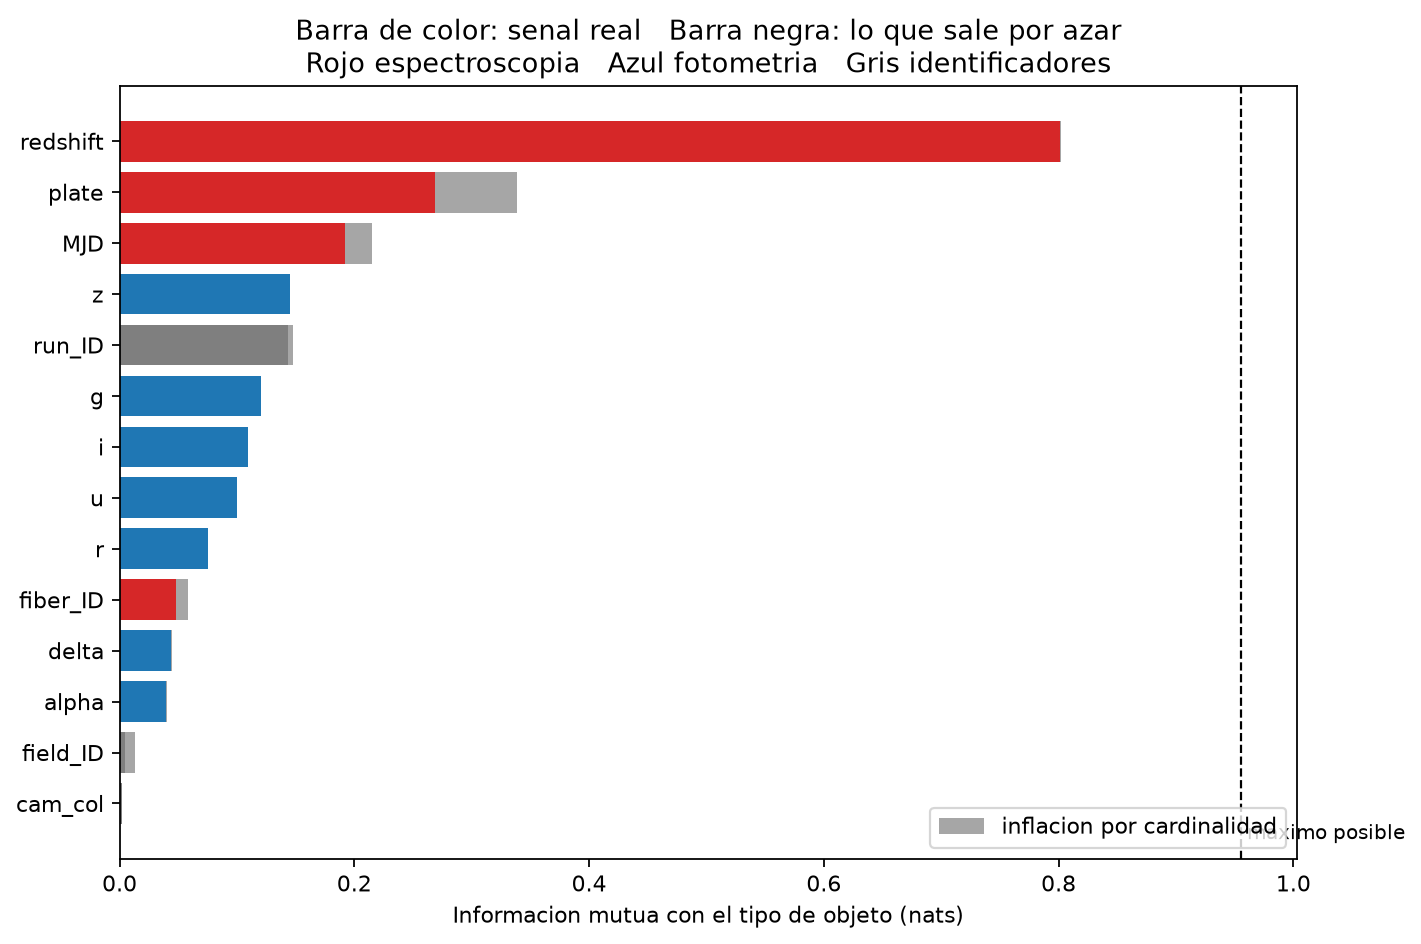
\includegraphics[width=\linewidth]{assets/images/fig_informacion_mutua.png}
    \caption{Informaci\'on mutua de cada columna con el tipo de objeto. La barra de color es el exceso sobre la l\'inea base por permutaci\'on; la barra negra es la inflaci\'on atribuible a la cardinalidad.}
    \label{fig:mi}
  \end{figure}

  Tres exclusiones se derivan de esta medici\'on, y ninguna se sostiene en que la variable sea poco informativa ---al contrario, las tres est\'an entre las m\'as informativas del cat\'alogo---:

  \textbf{\texttt{redshift} (exceso 0.8014 nats).} Concentra el 84\,\% de la entrop\'ia total de la etiqueta: por s\'i sola casi resuelve el problema. La raz\'on para excluirla no es esa magnitud, sino su procedencia. El \emph{pipeline} espectrosc\'opico del SDSS no mide el corrimiento al rojo y luego, por separado, clasifica el objeto: ajusta simult\'aneamente pares (plantilla de tipo $\times$ corrimiento) contra el espectro observado y se queda con la combinaci\'on de mejor $\chi^2$ \cite{bolton2012}. La inseparabilidad es de fondo, no de implementaci\'on: para medir cu\'anto se desplaz\'o una l\'inea espectral hay que saber qu\'e l\'inea es, y para identificarla hay que reconocer el patr\'on completo, que depende del tipo de objeto. \textbf{No se puede medir el corrimiento sin suponer qu\'e tipo de objeto es, ni determinar el tipo sin conocer el corrimiento.} Usar \texttt{redshift} como predictor equivaldr\'ia a alimentar al modelo con la respuesta ya calculada, el mismo tipo de fuga descrito en la literatura sobre \emph{leakage} \cite{kaufman2012}.

  \textbf{\texttt{plate} (0.2691), \texttt{MJD} (0.1920) y \texttt{run\_ID} (0.1432).} Superan a la mejor banda fotom\'etrica ($z$, 0.1449, y las tres primeras superan a $g$, $i$, $u$ y $r$). No son propiedades del objeto: identifican la placa met\'alica de fibras \'opticas, la fecha juliana modificada de la observaci\'on y la pasada del telescopio. Informan porque el sondeo \emph{decide} qu\'e observar y cu\'ando: una placa dedicada a un programa de cu\'asares contiene desproporcionadamente cu\'asares. Es un \textbf{efecto de selecci\'on} del sondeo, no f\'isica del objeto, y un modelo que lo aproveche estar\'ia aprendiendo el calendario del telescopio.

  El conjunto final de predictores qued\'o reducido a las \textbf{cinco magnitudes fotom\'etricas} $u$, $g$, $r$, $i$, $z$. Las coordenadas \texttt{alpha} y \texttt{delta} se excluyeron por la misma raz\'on de selecci\'on (informan sobre qu\'e regi\'on del cielo se prioriz\'o), y los identificadores restantes por carecer de contenido f\'isico.

  \subsection{Escalado}

  Las cinco bandas se estandarizaron con \texttt{StandardScaler} ($z=(x-\mu)/\sigma$) antes del PCA. Aunque las magnitudes comparten unidad y rango similar, el PCA diagonaliza la matriz de covarianza y por tanto es sensible a la escala de cada variable: sin estandarizar, la banda de mayor varianza dominar\'ia el primer componente por una raz\'on aritm\'etica y no informativa \cite{jolliffe2016}.

  \section{Metodolog\'ia}

  \subsection{An\'alisis de Componentes Principales}

  PCA busca un nuevo sistema de ejes, rotaci\'on del original, tal que el primer eje capture la mayor varianza posible, el segundo la mayor varianza restante siendo ortogonal al primero, y as\'i sucesivamente. Formalmente, los ejes son los vectores propios $\mathbf{w}$ de la matriz de covarianza $\Sigma$ de los datos estandarizados:
  \begin{equation}
    \Sigma \mathbf{w}_j = \lambda_j \mathbf{w}_j, \qquad \lambda_1 \geq \lambda_2 \geq \dots \geq \lambda_p
    \label{eq:pca}
  \end{equation}
  donde el valor propio $\lambda_j$ es la varianza capturada por el eje $j$, y la proporci\'on $\lambda_j / \sum_i \lambda_i$ es la \emph{varianza explicada} \cite{hotelling1933,jolliffe2016}. Los coeficientes de cada vector propio (\emph{loadings}) indican cu\'anto pesa cada variable original dentro del componente, y son lo que permite interpretarlo f\'isicamente.

  Debe subrayarse un punto que resulta decisivo en la Secci\'on~\ref{sec:resultados}: \textbf{PCA maximiza varianza, no separabilidad}. Nada en la Ecuaci\'on~\ref{eq:pca} involucra la etiqueta, de modo que no existe garant\'ia alguna de que el eje de mayor varianza sea el m\'as \'util para distinguir clases.

  \subsection{K-medias}

  K-medias parte los datos en $k$ grupos minimizando la suma de distancias euclidianas al cuadrado entre cada punto y el centroide de su grupo \cite{macqueen1967,lloyd1982}:
  \begin{equation}
    J = \sum_{j=1}^{k} \sum_{\mathbf{x} \in C_j} \lVert \mathbf{x} - \boldsymbol{\mu}_j \rVert^2
    \label{eq:kmeans}
  \end{equation}
  El algoritmo alterna dos pasos hasta converger: asignar cada punto al centroide m\'as cercano, y recalcular cada centroide como la media de sus puntos. La consecuencia geom\'etrica de usar distancia euclidiana es que \textbf{K-medias supone grupos esf\'ericos y de tama\~no comparable}: sus fronteras son hiperplanos equidistantes entre centroides (una teselaci\'on de Voronoi). Un grupo genuinamente alargado o inclinado no puede representarse con ese vocabulario.

  \subsection{Mezcla de Gaussianas}

  Una mezcla gaussiana modela la densidad de los datos como suma ponderada de $k$ campanas multivariadas \cite{mclachlan2000}:
  \begin{equation}
    p(\mathbf{x}) = \sum_{j=1}^{k} \pi_j \, \mathcal{N}(\mathbf{x} \mid \boldsymbol{\mu}_j, \Sigma_j), \qquad \sum_{j=1}^{k} \pi_j = 1
    \label{eq:gmm}
  \end{equation}
  Los par\'ametros se ajustan por m\'axima verosimilitud con el algoritmo EM \cite{dempster1977,hastie2009}, que alterna entre calcular la probabilidad de que cada punto pertenezca a cada campana (\emph{responsabilidades}) y reestimar medias, covarianzas y pesos con esas probabilidades como ponderaci\'on. A diferencia de K-medias, la asignaci\'on es \textbf{blanda}: cada objeto recibe una distribuci\'on de pertenencia, no una etiqueta dura.

  La diferencia geom\'etrica de fondo est\'a en la m\'etrica. La pertenencia a una campana no depende de la distancia euclidiana al centro sino de la \textbf{distancia de Mahalanobis} \cite{mahalanobis1936}:
  \begin{equation}
    d_M^2(\mathbf{x}, \boldsymbol{\mu}_j) = (\mathbf{x} - \boldsymbol{\mu}_j)^{\top} \Sigma_j^{-1} (\mathbf{x} - \boldsymbol{\mu}_j)
    \label{eq:mahalanobis}
  \end{equation}
  que mide el desplazamiento en unidades de la dispersi\'on propia del grupo \emph{en cada direcci\'on}. Dos puntos a la misma distancia euclidiana del centro pueden estar a distancias de Mahalanobis muy distintas si la campana es alargada. Cuando $\Sigma_j = \sigma^2 I$, la Ecuaci\'on~\ref{eq:mahalanobis} se reduce a la distancia euclidiana escalada y la mezcla se comporta como K-medias.

  La forma admisible de $\Sigma_j$ se controla con el par\'ametro \texttt{covariance\_type}, que en \texttt{scikit-learn} ofrece cuatro variantes crecientes en libertad \cite{pedregosa2011}: \texttt{spherical} (una sola varianza por campana), \texttt{tied} (una \'unica matriz completa compartida por todas), \texttt{diag} (una matriz diagonal por campana, ejes independientes pero alineados con los del espacio) y \texttt{full} (una matriz completa por campana, con inclinaci\'on propia).

  \subsection{M\'etricas de Evaluaci\'on}

  Sin etiqueta no hay \emph{accuracy}, por lo que la evaluaci\'on combina tres criterios de naturaleza distinta.

  \textbf{Silhouette} (criterio \emph{interno}): mide qu\'e tan compacto y separado qued\'o cada grupo usando \'unicamente la geometr\'ia de los datos \cite{rousseeuw1987}. Para cada punto $i$, con $a(i)$ la distancia media a los puntos de su propio grupo y $b(i)$ la distancia media al grupo vecino m\'as cercano:
  \begin{equation}
    s(i) = \frac{b(i) - a(i)}{\max\{a(i), b(i)\}} \in [-1, 1]
    \label{eq:silhouette}
  \end{equation}

  \textbf{Informaci\'on Mutua Ajustada} (criterio \emph{externo}): compara la partici\'on hallada $U$ con la etiqueta real $V$, corrigiendo por el acuerdo esperado al azar \cite{vinh2010}:
  \begin{equation}
    AMI(U,V) = \frac{MI(U,V) - \mathbb{E}[MI(U,V)]}{\overline{H}(U,V) - \mathbb{E}[MI(U,V)]}
    \label{eq:ami}
  \end{equation}
  Vale 0 cuando la coincidencia es la esperable por azar y 1 cuando las particiones son id\'enticas. La correcci\'on por azar importa aqu\'i: sin ella, dos particiones cualesquiera con muchos grupos parecen coincidir m\'as de lo que realmente lo hacen.

  \textbf{Criterio de Informaci\'on Bayesiano} (BIC), para elegir entre modelos de la misma familia probabil\'istica \cite{schwarz1978}:
  \begin{equation}
    BIC = -2 \ln \hat{L} + p \ln n
    \label{eq:bic}
  \end{equation}
  Penaliza la verosimilitud $\hat{L}$ por el n\'umero de par\'ametros $p$; a menor BIC, mejor. Es aplicable a las variantes de GMM entre s\'i, pero \textbf{no} a K-medias, que no define una verosimilitud comparable.

  Es indispensable subrayar que el AMI \textbf{usa la etiqueta}. En un problema genuinamente sin etiquetar no estar\'ia disponible, y ese es el l\'imite honesto de este trabajo: se dispone de una vara externa que en la pr\'actica no se tendr\'ia.

  \section{Resultados y Discusi\'on}
  \label{sec:resultados}

  \subsection{PCA: la varianza no es la utilidad}
  \label{sec:pca}

  El PCA sobre las cinco bandas estandarizadas produce una reducci\'on muy eficiente en t\'erminos de varianza: PC1 concentra el 85.63\,\%, PC2 el 11.77\,\% y PC3 el 1.86\,\%, de modo que dos componentes acumulan el 97.40\,\% y tres el 99.26\,\% (Figura~\ref{fig:pca}, izquierda).

  \begin{figure*}[t]
    \centering
    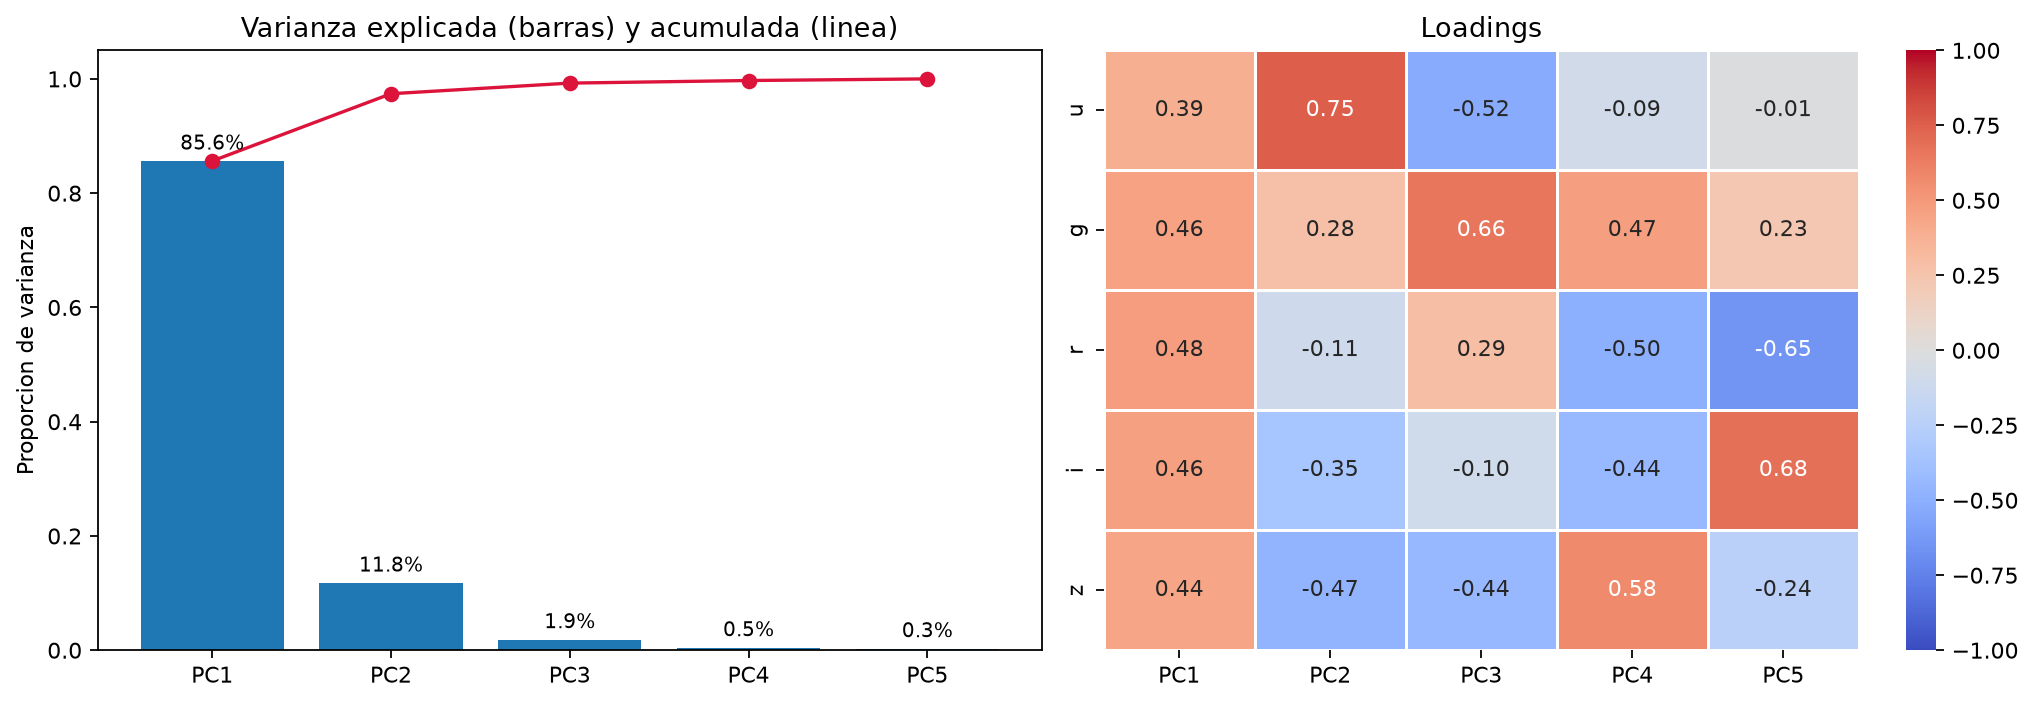
\includegraphics[width=0.85\linewidth]{assets/images/fig_pca_varianza_loadings.png}
    \caption{Varianza explicada y acumulada (izquierda) y \emph{loadings} de cada banda en cada componente (derecha).}
    \label{fig:pca}
  \end{figure*}

  Los \emph{loadings} (Figura~\ref{fig:pca}, derecha) permiten leer f\'isicamente los dos primeros ejes. En PC1 las cinco bandas pesan con el mismo signo y magnitudes parecidas (entre 0.387 y 0.477): es un promedio de las cinco magnitudes, es decir, \textbf{el brillo global del objeto}. En PC2 los signos se separan de forma ordenada por longitud de onda ($u$: $+0.754$, $g$: $+0.280$, $r$: $-0.107$, $i$: $-0.346$, $z$: $-0.471$): es un contraste entre el extremo azul y el extremo rojo del espectro, es decir, \textbf{el color}.

  El resultado central del an\'alisis aparece al confrontar varianza con informaci\'on (Figura~\ref{fig:varianzami}, izquierda). El componente que acumula el 85.63\,\% de la varianza queda cuarto de cinco en informaci\'on mutua con el tipo de objeto (MI $=0.0677$ nats), mientras que PC2, con apenas el 11.77\,\% de la varianza, es el m\'as informativo (MI $=0.2942$ nats, m\'as del cu\'adruple que PC1). PC3 (1.86\,\% de varianza) informa 0.0800, tambi\'en por encima de PC1, e incluso PC4 (0.45\,\% de varianza) alcanza 0.0861.

  \begin{figure*}[t]
    \centering
    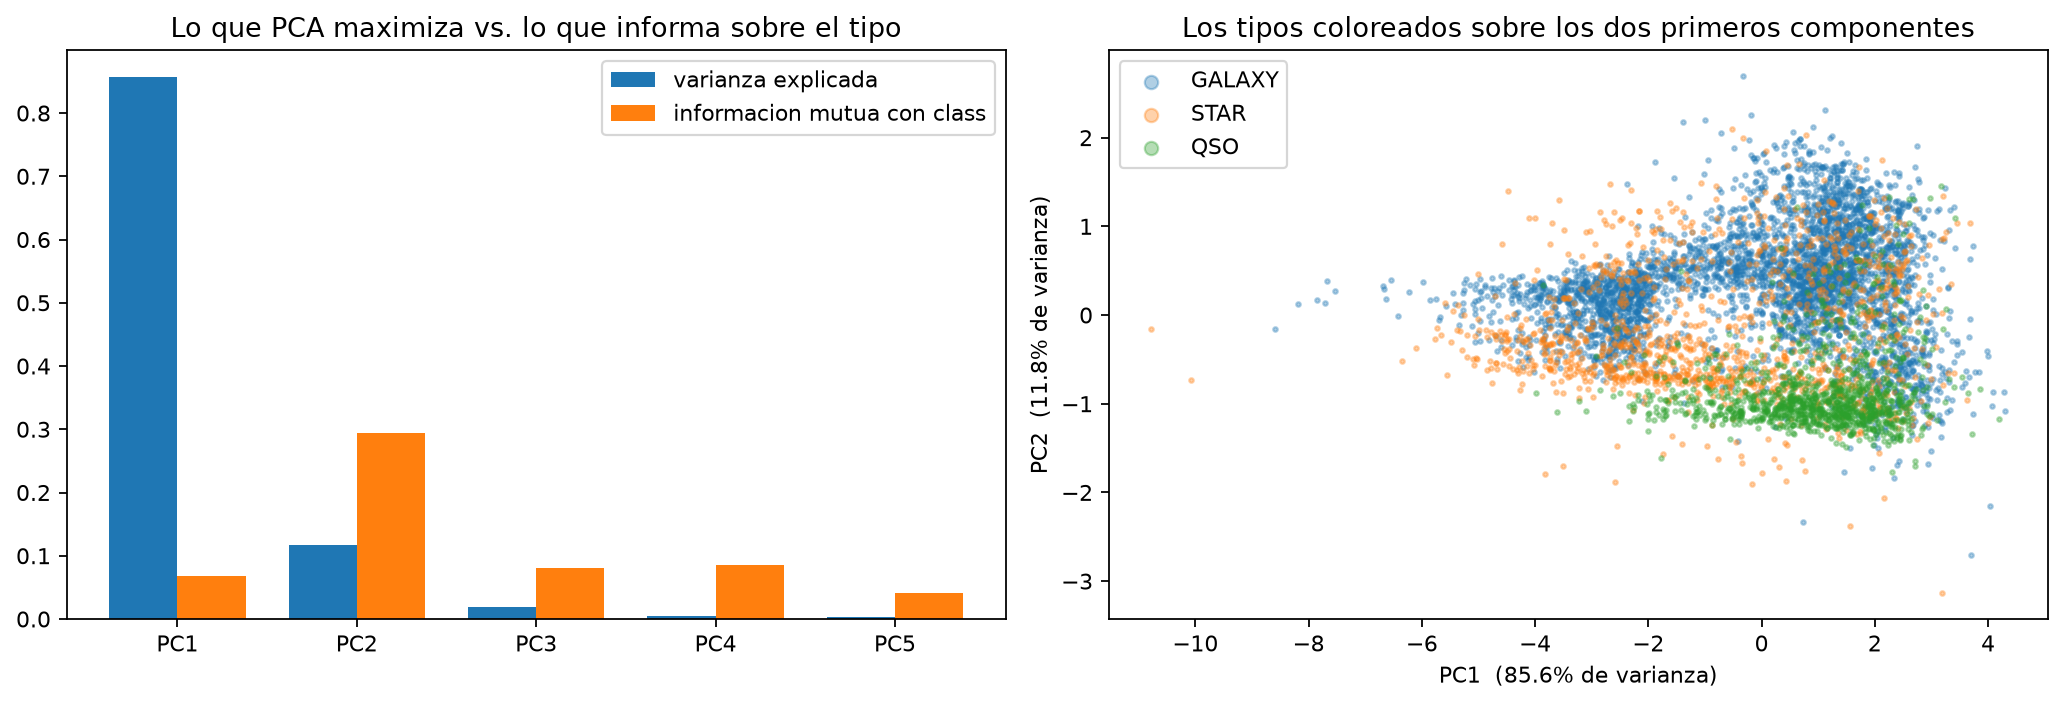
\includegraphics[width=0.85\linewidth]{assets/images/fig_varianza_vs_informacion.png}
    \caption{Izquierda: varianza explicada frente a informaci\'on mutua con el tipo, por componente. Derecha: los tres tipos reales proyectados sobre PC1--PC2 (muestra de 6\,000 objetos).}
    \label{fig:varianzami}
  \end{figure*}

  La interpretaci\'on f\'isica de esta disociaci\'on es directa y consistente con lo dicho en la Introducci\'on. La mayor fuente de variabilidad en un cat\'alogo fotom\'etrico es el brillo aparente, que depende sobre todo de la distancia: hay objetos cercanos y objetos lejanos de todos los tipos. El color, en cambio, describe la forma del espectro y es lo que distingue f\'isicamente a una estrella de un cu\'asar. La dispersi\'on de la Figura~\ref{fig:varianzami} (derecha) lo confirma visualmente: los tres tipos se solapan ampliamente a lo largo de PC1 y se ordenan, con solapamiento pero de forma perceptible, a lo largo de PC2.

  \textbf{Esta es la advertencia metodol\'ogica m\'as importante del trabajo}: elegir componentes por varianza acumulada ---el procedimiento habitual, y el \'unico disponible sin etiqueta--- habr\'ia conservado los dos primeros (97.4\,\%) y descartado precisamente componentes que informan m\'as que el que se conserv\'o primero.

  \subsection{Selecci\'on de componentes y de $k$}

  Con $k=3$ fijo, el barrido sobre el n\'umero de componentes retenidos muestra un comportamiento muy asim\'etrico entre los dos algoritmos (Tabla~\ref{tab:componentes}). K-medias es indiferente: su AMI se mantiene plano en $\approx 0.047$ con dos, tres o cuatro componentes. La mezcla gaussiana, en cambio, salta de 0.0584 a 0.2434 al pasar de dos a tres componentes, y vuelve a caer a 0.0548 con cuatro.

  \begin{table}[H]
    \caption{Efecto del n\'umero de componentes retenidos, con $k=3$ fijo}
    \label{tab:componentes}
    \centering
    \begin{tabular}{cccc}
      \toprule
      \textbf{Componentes} & \textbf{Var. acumulada} & \textbf{AMI K-medias} & \textbf{AMI GMM} \\
      \midrule
      2 & 0.9740 & 0.0474 & 0.0584 \\
      3 & 0.9926 & 0.0473 & \textbf{0.2434} \\
      4 & 0.9972 & 0.0472 & 0.0548 \\
      \bottomrule
    \end{tabular}
  \end{table}

  Debe declararse con claridad que \textbf{la columna que se\~nala a tres componentes como la mejor opci\'on es el AMI, y el AMI se calcula contra la etiqueta}. En un problema realmente sin etiquetar solo se dispondr\'ia de la varianza acumulada, se habr\'ian elegido dos componentes, y nunca se habr\'ia sabido lo que se perd\'ia. La configuraci\'on ganadora se eligi\'o mirando la respuesta.

  Para el n\'umero de grupos se fij\'o $k=3$ por dos razones convergentes: es el n\'umero de clases de la etiqueta de referencia, lo que hace comparables las particiones, y los criterios internos no ofrecen una alternativa concluyente (Figura~\ref{fig:seleccionk}). La inercia decrece suavemente sin codo n\'itido; el silhouette es m\'aximo en $k=2$ (0.5607) y cae a 0.3800 en $k=3$; y el BIC de la mezcla decrece de forma mon\'otona hasta $k=8$ sin encontrar m\'inimo en el rango explorado. Es decir, ning\'un criterio interno apunta a tres grupos: la elecci\'on se apoya en el conocimiento de la etiqueta, no en la geometr\'ia.

  \begin{figure*}[t]
    \centering
    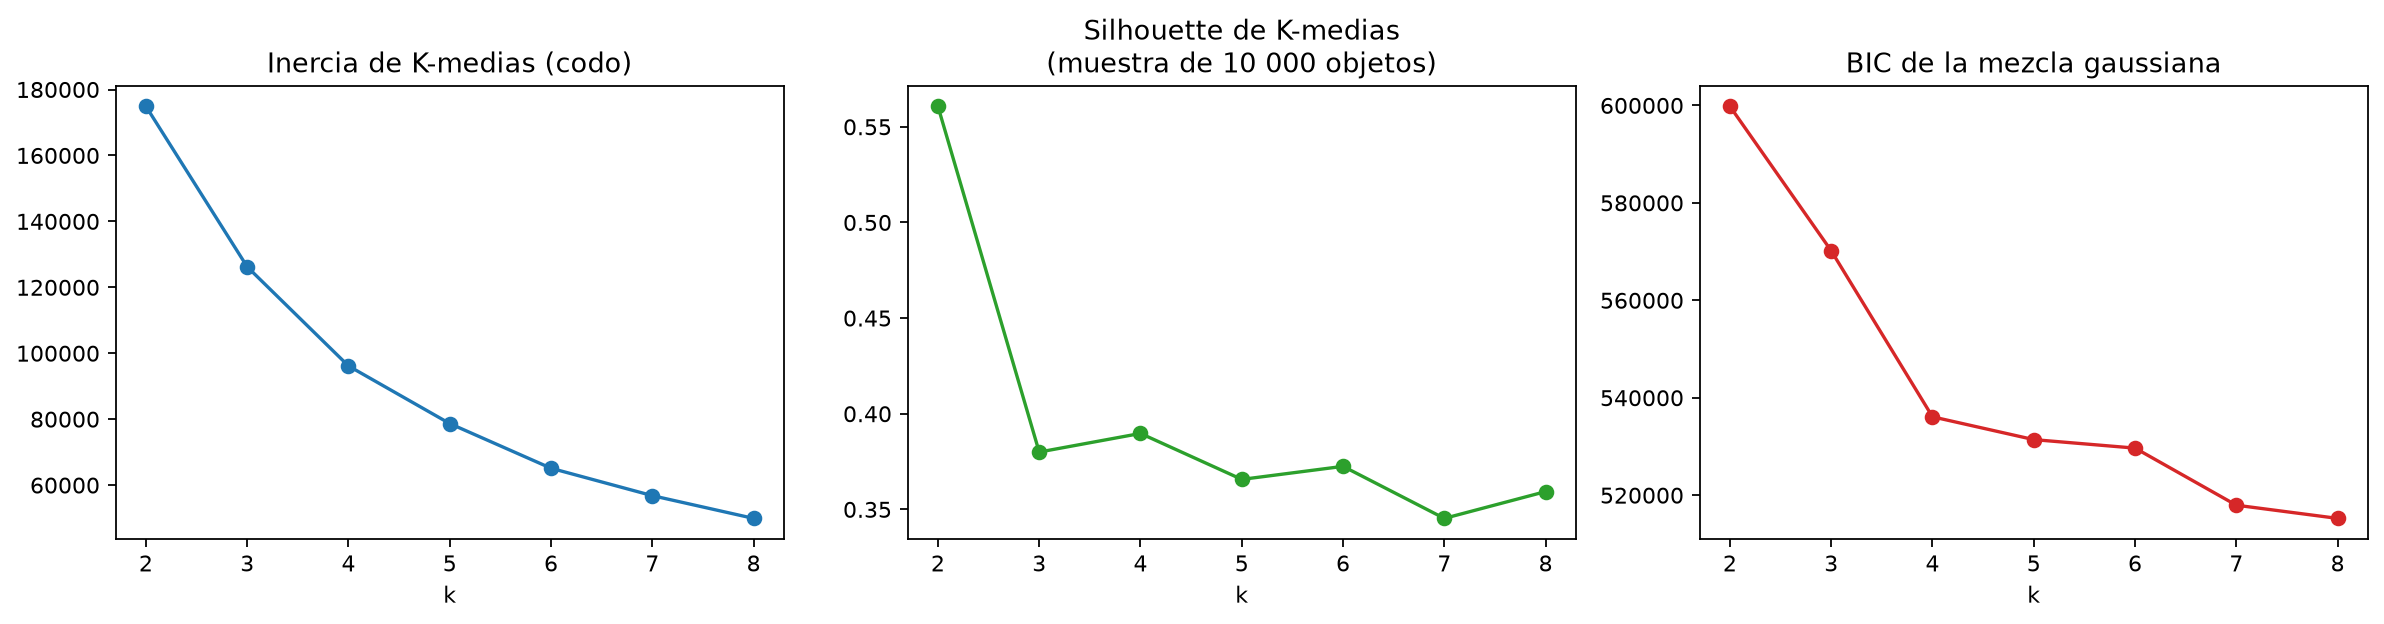
\includegraphics[width=0.9\linewidth]{assets/images/fig_seleccion_k.png}
    \caption{Criterios para elegir $k$: inercia de K-medias, silhouette y BIC de la mezcla gaussiana. Ninguno se\~nala $k=3$.}
    \label{fig:seleccionk}
  \end{figure*}

  \subsection{Qu\'e eje usa realmente cada algoritmo}
  \label{sec:ejes}

  La diferencia de comportamiento entre los dos modelos se explica al inspeccionar sus centroides. Midiendo el rango que cubren los tres centros en cada eje, K-medias los separa 4.76 unidades en PC1, 0.11 en PC2 y 0.04 en PC3: \textbf{parte los datos exclusivamente por brillo}, ignorando el color por completo. Las medias de la mezcla gaussiana, en cambio, se reparten 3.91 en PC1 pero tambi\'en 1.44 en PC2, un orden de magnitud m\'as que K-medias.

  La Tabla~\ref{tab:subconjuntos} pone a prueba esta lectura entregando a cada algoritmo distintos subconjuntos de ejes. El experimento confirma el diagn\'ostico: K-medias sobre PC1 solo (0.0478) rinde lo mismo que sobre los tres ejes juntos (0.0473), mientras que K-medias sobre PC2 solo salta a 0.2014. Cuando se le retira PC1 y se le deja PC2+PC3, K-medias alcanza 0.2093, cuatro veces su desempe\~no con todos los ejes disponibles. \textbf{El componente de mayor varianza no solo no ayudaba: activamente estorbaba}, porque su escala domina la distancia euclidiana de la Ecuaci\'on~\ref{eq:kmeans} y arrastra la partici\'on hacia \'el.

  \begin{table}[H]
    \caption{AMI seg\'un los ejes entregados a cada algoritmo}
    \label{tab:subconjuntos}
    \centering
    \resizebox{\linewidth}{!}{%
      \begin{tabular}{lcccc}
        \toprule
        \textbf{Ejes usados} & \textbf{Var. incl.} & \textbf{K-medias} & \textbf{GMM diag} & \textbf{GMM full} \\
        \midrule
        PC1          & 0.8563 & 0.0478 & 0.0456 & 0.0456 \\
        PC2          & 0.1177 & 0.2014 & 0.2012 & 0.2012 \\
        PC3          & 0.0186 & 0.0302 & 0.0268 & 0.0268 \\
        PC1+PC2      & 0.9740 & 0.0474 & 0.0529 & 0.0584 \\
        PC1+PC3      & 0.8749 & 0.0484 & 0.0427 & 0.0499 \\
        PC2+PC3      & 0.1363 & \textbf{0.2093} & 0.2095 & 0.1403 \\
        PC1+PC2+PC3  & 0.9926 & 0.0473 & 0.1441 & \textbf{0.2434} \\
        \bottomrule
      \end{tabular}%
    }
  \end{table}

  La mezcla gaussiana con covarianza \texttt{full} sobre los tres componentes es la \'unica configuraci\'on que supera lo que se obtiene descartando PC1 a mano: 0.2434 frente a 0.2095, el mejor valor de la fila PC2+PC3. Es decir, \textbf{el modelo probabil\'istico logra convivir con el eje de brillo en lugar de tener que eliminarlo}, porque la Ecuaci\'on~\ref{eq:mahalanobis} le permite normalizar internamente la dispersi\'on de cada direcci\'on en vez de sufrirla.

  \subsection{El efecto de \texttt{covariance\_type}}
  \label{sec:covtype}

  Manteniendo fijos los tres componentes y $k=3$, variar \'unicamente la forma admisible de las campanas produce una progresi\'on mon\'otona en el criterio externo (Tabla~\ref{tab:covtype}): \texttt{spherical} 0.0490, \texttt{tied} 0.0750, \texttt{diag} 0.1441, \texttt{full} 0.2434. La variante m\'as restringida es indistinguible de K-medias (0.0473), lo cual es coherente con la teor\'ia: K-medias se obtiene como el l\'imite de una mezcla de gaussianas esf\'ericas cuando la varianza com\'un tiende a cero y las responsabilidades se vuelven duras \cite[\S9.3.2]{bishop2006}.

  \begin{table}[H]
    \caption{Comparaci\'on de \texttt{covariance\_type} con $k=3$ y tres componentes}
    \label{tab:covtype}
    \centering
    \resizebox{\linewidth}{!}{%
      \begin{tabular}{lcccc}
        \toprule
        \textbf{Variante} & \textbf{Par\'ams.} & \textbf{BIC} & \textbf{Silhouette} & \textbf{AMI} \\
        \midrule
        \texttt{spherical} & 14 & 783\,501 & \textbf{0.3823} & 0.0490 \\
        \texttt{tied}      & 17 & 660\,495 & 0.3271 & 0.0750 \\
        \texttt{diag}      & 20 & 604\,604 & 0.3025 & 0.1441 \\
        \texttt{full}      & 29 & \textbf{570\,165} & 0.3619 & \textbf{0.2434} \\
        \midrule
        K-medias (ref.)    & --- & --- & 0.3800 & 0.0473 \\
        \bottomrule
      \end{tabular}%
    }
  \end{table}

  La Figura~\ref{fig:covtype} muestra el hallazgo m\'as inc\'omodo del experimento: \textbf{los dos criterios de evaluaci\'on no coinciden}. El mejor modelo seg\'un el silhouette es \texttt{spherical}, que es de los peores seg\'un el AMI; y \texttt{full}, el mejor por AMI, queda segundo por silhouette, por debajo de la variante que peor recupera la estructura real. La explicaci\'on es que el silhouette premia grupos compactos y bien separados en distancia euclidiana ---exactamente el tipo de partici\'on que produce cortar por PC1---, mientras que la estructura f\'isica real vive en un eje de baja varianza. El BIC, en cambio, s\'i ordena igual que el AMI en este caso, pero eso no lo convierte en un criterio confiable en general: mide ajuste de densidad, no correspondencia con una taxonom\'ia.

  \begin{figure}[H]
    \centering
    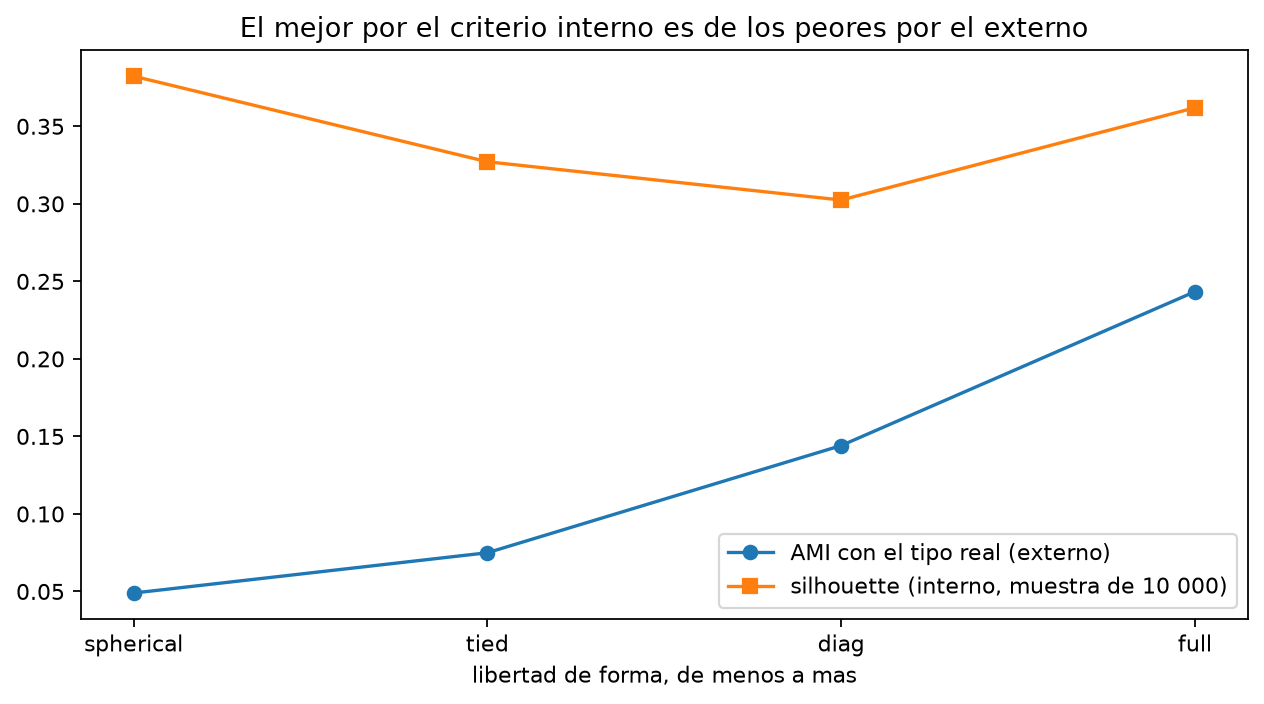
\includegraphics[width=\linewidth]{assets/images/fig_covariance_type.png}
    \caption{AMI (externo) y silhouette (interno) a lo largo de las cuatro variantes de \texttt{covariance\_type}. Los dos criterios se\~nalan ganadores distintos.}
    \label{fig:covtype}
  \end{figure}

  \subsubsection{Tres libertades, no una}

  Resulta tentador atribuir la ventaja de \texttt{full} a una \'unica propiedad geom\'etrica, pero la tabla no lo permite. Las cuatro variantes se distinguen por \emph{tres} libertades independientes: si cada campana tiene matriz propia, si puede tener ancho distinto por eje, y si puede inclinarse respecto a los ejes del espacio. \texttt{tied} tiene inclinaci\'on pero no matriz propia por grupo (0.0750); \texttt{diag} tiene matriz propia y ancho por eje pero no inclinaci\'on (0.1441). Ninguna de las dos libertades por separado explica el salto: hace falta la combinaci\'on completa.

  La geometr\'ia ajustada lo ilustra. En \texttt{diag} las tres campanas quedan con alargamientos de 2.0, 15.4 y 10.1, todas necesariamente a $0^{\circ}$; en \texttt{full} los alargamientos son 9.7, 16.7 y 2.6 con inclinaciones de $2.8^{\circ}$, $5.4^{\circ}$ y $13.4^{\circ}$. Los anchos a lo largo de PC1 son similares entre las tres campanas de \texttt{full} (1.35, 1.22 y 1.02), mientras que a lo largo de PC2 difieren mucho m\'as (0.26, 0.43 y 0.62).

  Debe consignarse con honestidad el l\'imite de este an\'alisis: \textbf{el mecanismo fino no qued\'o aislado}. Los experimentos permiten mostrar \emph{que} el salto ocurre y acotar \emph{de qu\'e libertades depende}, pero no derivar el \emph{porqu\'e} \'ultimo a partir de las magnitudes medidas. Varias hip\'otesis intermedias que se formularon durante el an\'alisis ---que la ventaja proven\'ia de explotar la correlaci\'on entre PC1 y PC3, o de estirar cada campana de forma distinta a lo largo de PC1--- fueron contrastadas y descartadas por los propios datos.

  \subsubsection{Estabilidad}

  Ninguno de los resultados anteriores depende del azar de la inicializaci\'on. Sobre ocho semillas distintas, el AMI de la mezcla \texttt{full} sobre tres componentes tiene media 0.2434 y desviaci\'on est\'andar 0.0001 (rango 0.2432--0.2435), y el de K-medias sobre PC2+PC3 media 0.2092 con desviaci\'on 0.0002 (rango 0.2090--0.2093).

  \subsection{Una representaci\'on alternativa: colores en vez de bandas}

  Dado que la f\'isica apunta al color y no al brillo, se prob\'o construir el espacio directamente sobre las cuatro diferencias consecutivas $u-g$, $g-r$, $r-i$, $i-z$, en lugar de sobre las cinco magnitudes. El cambio altera la geometr\'ia por completo: la varianza deja de concentrarse (PC1 baja de 85.6\,\% a 47.3\,\%) y los centroides de K-medias pasan a repartirse 2.53 en PC1, 1.72 en PC2 y 0.77 en PC3, en vez de concentrarse en un solo eje.

  \begin{table}[H]
    \caption{Comparaci\'on de representaciones y modelos ($k=3$, tres componentes)}
    \label{tab:representaciones}
    \centering
    \resizebox{\linewidth}{!}{%
      \begin{tabular}{llcc}
        \toprule
        \textbf{Representaci\'on} & \textbf{Modelo} & \textbf{Silhouette} & \textbf{AMI} \\
        \midrule
        PCA sobre bandas  & K-medias         & 0.3800 & 0.0473 \\
        PCA sobre bandas  & Mezcla gaussiana & 0.3619 & \textbf{0.2434} \\
        PCA sobre colores & K-medias         & \textbf{0.3876} & 0.1775 \\
        PCA sobre colores & Mezcla gaussiana & 0.2787 & 0.1243 \\
        \bottomrule
      \end{tabular}%
    }
  \end{table}

  El efecto sobre K-medias es notable: pasa de 0.0473 a 0.1775, casi cuatro veces mejor, simplemente por cambiar la representaci\'on de entrada sin tocar el algoritmo. \textbf{Preparar el espacio result\'o m\'as decisivo para K-medias que cualquier ajuste de sus hiperpar\'ametros.} Sobre la mezcla gaussiana, en cambio, el mismo cambio es contraproducente (0.2434 $\to$ 0.1243). Esto es coherente con lo observado en la Secci\'on~\ref{sec:ejes}: su ventaja consist\'ia en \emph{neutralizar} el eje de brillo, no en extraer informaci\'on de \'el. Removido ese eje de la representaci\'on, la flexibilidad extra de la covarianza completa deja de compensar y pasa a ser un costo, porque lo que ajusta es \textbf{densidad} y no separaci\'on de clases. La conclusi\'on no es que una representaci\'on sea mejor, sino que \textbf{representaci\'on y modelo deben elegirse juntos}. La Figura~\ref{fig:representaciones} confirma adem\'as que los dos criterios siguen sin coincidir: la mejor combinaci\'on por silhouette (colores + K-medias, 0.3876) no es la mejor por AMI.

  \begin{figure*}[t]
    \centering
    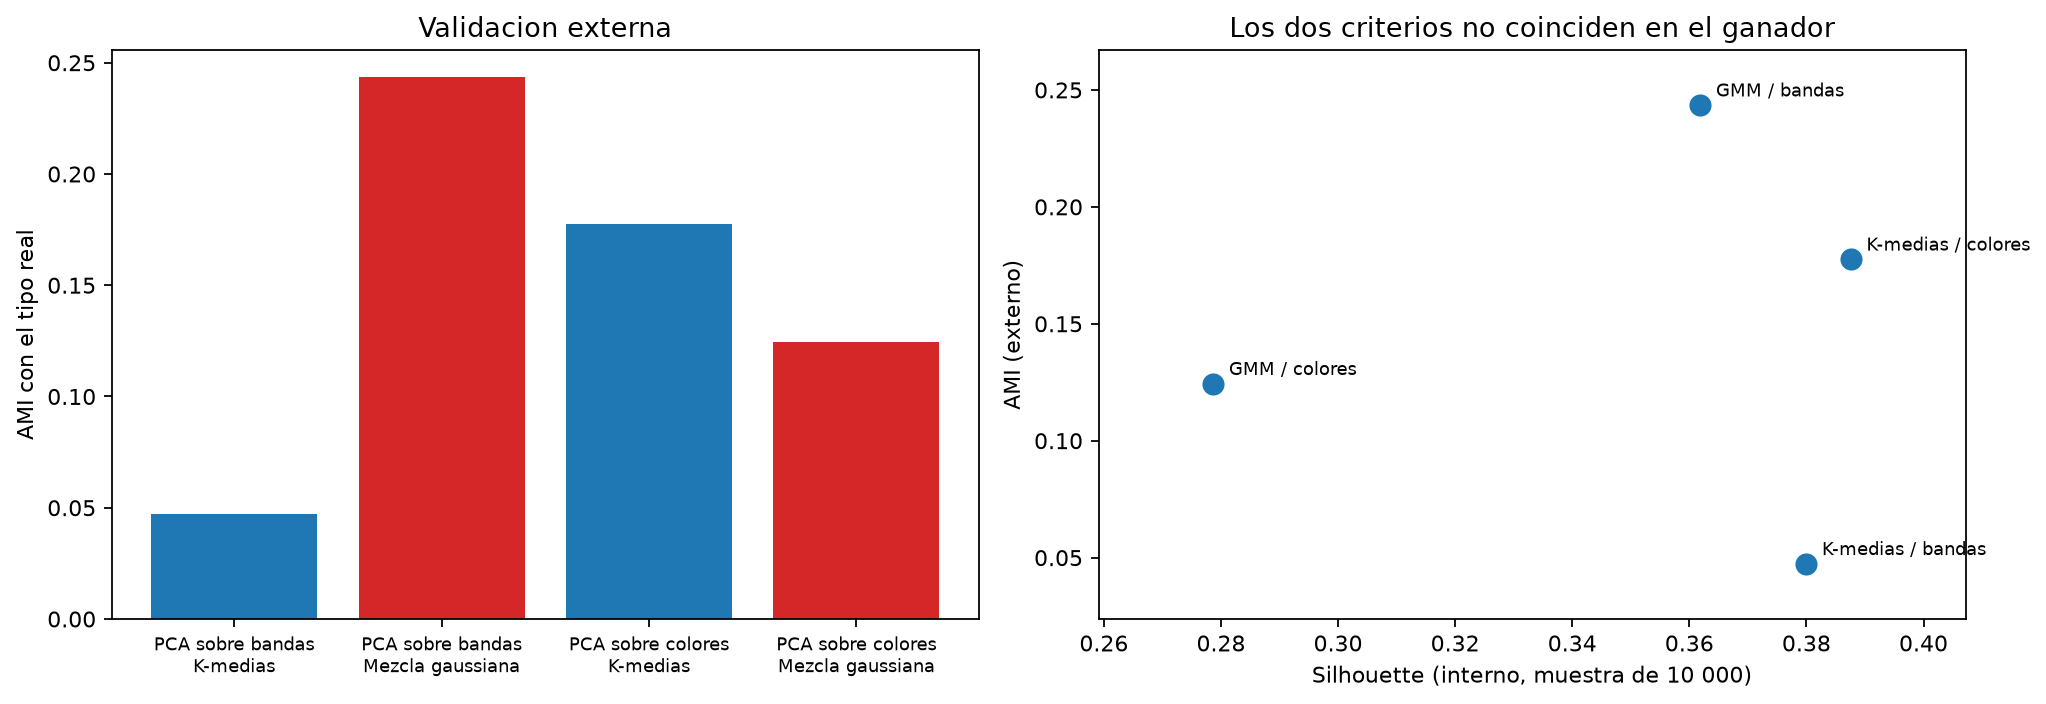
\includegraphics[width=0.85\linewidth]{assets/images/fig_representaciones.png}
    \caption{Izquierda: AMI de las cuatro combinaciones de representaci\'on y modelo. Derecha: cada combinaci\'on situada sobre los dos criterios de evaluaci\'on a la vez.}
    \label{fig:representaciones}
  \end{figure*}

  \subsection{Qu\'e encontr\'o realmente el mejor modelo}
  \label{sec:mejormodelo}

  Un AMI de 0.2434 es un n\'umero abstracto; la tabla de contingencia dice qu\'e significa. La Figura~\ref{fig:grupos} la presenta en sus dos lecturas complementarias, junto con la distribuci\'on de certeza del modelo. Leyendo por fila ---a d\'onde fue a parar cada tipo real--- el comportamiento es muy desigual entre las tres clases:

  \begin{figure*}[t]
    \centering
    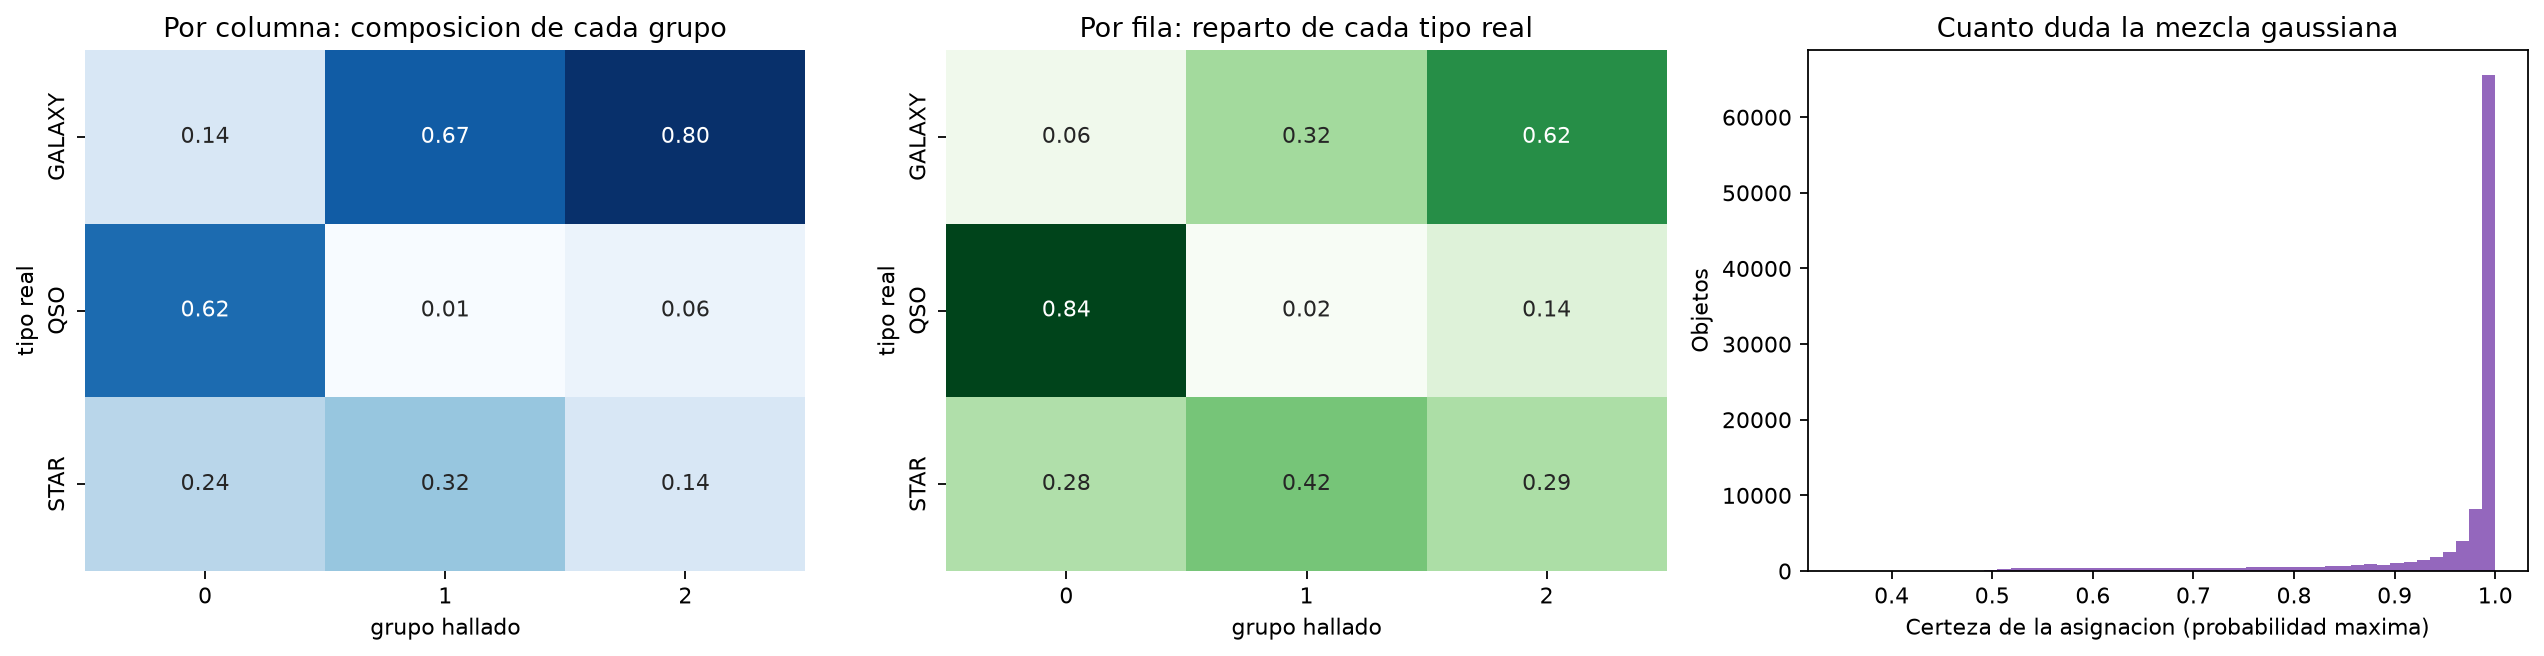
\includegraphics[width=0.85\linewidth]{assets/images/fig_grupos_vs_tipos.png}
    \caption{Composici\'on de los grupos hallados por la mezcla gaussiana \texttt{full}. Izquierda: de qu\'e est\'a hecho cada grupo. Centro: a d\'onde fue a parar cada tipo real. Derecha: distribuci\'on de la certeza de asignaci\'on.}
    \label{fig:grupos}
  \end{figure*}

  \begin{table}[H]
    \caption{Reparto de cada tipo real entre los tres grupos hallados (por fila)}
    \label{tab:crosstab}
    \centering
    \begin{tabular}{lccc}
      \toprule
      \textbf{Tipo real} & \textbf{Grupo 0} & \textbf{Grupo 1} & \textbf{Grupo 2} \\
      \midrule
      \texttt{GALAXY} & 0.059 & 0.319 & \textbf{0.623} \\
      \texttt{QSO}    & \textbf{0.840} & 0.016 & 0.144 \\
      \texttt{STAR}   & 0.284 & \textbf{0.423} & 0.293 \\
      \bottomrule
    \end{tabular}
  \end{table}

  Los cu\'asares son el \'exito claro: el 84.0\,\% cae en un mismo grupo, que adem\'as est\'a compuesto en un 62.4\,\% por cu\'asares. Tiene sentido f\'isico, porque un cu\'asar tiene un espectro muy distintivo y por tanto un color muy caracter\'istico. Las galaxias quedan mayoritariamente en un grupo (62.3\,\%) pero con una fuga importante. Las estrellas son el fracaso: se reparten casi uniformemente entre los tres grupos (0.284 / 0.423 / 0.293), es decir, \textbf{el modelo no las distingue en absoluto}.

  El \'ultimo hallazgo es el m\'as instructivo desde el punto de vista metodol\'ogico. La mezcla asigna 85\,429 de los 99\,999 objetos (85.4\,\%) con una probabilidad m\'axima superior al 90\,\%, es decir, con muy poca duda. Restringido a esos objetos ``seguros'', el AMI sube apenas de 0.2434 a 0.2890. \textbf{La certeza del modelo y su correspondencia con la realidad son dos cosas distintas}: el modelo est\'a seguro y equivocado a la vez, porque la probabilidad que reporta mide el ajuste a las campanas que \'el mismo ajust\'o, no el acuerdo con la f\'isica.

  \FloatBarrier

  \section{Conclusiones}

  \begin{enumerate}
    \item \textbf{La varianza no es la utilidad.} El componente principal que concentra el 85.6\,\% de la varianza queda cuarto de cinco en informaci\'on mutua con el tipo de objeto (0.068 nats), mientras que el segundo, con 11.8\,\% de varianza, es el m\'as informativo (0.294). Elegir componentes por varianza acumulada ---el \'unico criterio disponible sin etiqueta--- habr\'ia descartado se\~nal \'util y conservado ruido dominante.
    \item \textbf{El supuesto geom\'etrico del algoritmo determin\'o el resultado m\'as que cualquier hiperpar\'ametro.} K-medias, atado a la distancia euclidiana, parti\'o los datos exclusivamente por brillo (separaci\'on de centroides: 4.76 en PC1 frente a 0.11 en PC2) y qued\'o en $AMI=0.0473$. La mezcla gaussiana con covarianza \texttt{full}, que mide en distancia de Mahalanobis, alcanz\'o $AMI=0.2434$ sobre los mismos datos.
    \item \textbf{La ventaja de \texttt{full} depende de tres libertades combinadas}, no de una sola: matriz propia por grupo, ancho propio por eje e inclinaci\'on. El mecanismo fino no se logr\'o aislar, y varias hip\'otesis intermedias fueron descartadas por los propios datos; se reporta el efecto medido, no una explicaci\'on que los experimentos no sostienen.
    \item \textbf{Los criterios interno y externo no coinciden.} El mejor modelo por silhouette (\texttt{spherical}) es de los peores por AMI. Sin etiqueta solo se dispondr\'ia del silhouette, y este habr\'ia se\~nalado el modelo equivocado. Es el l\'imite estructural del aprendizaje no supervisado, no un defecto del experimento.
    \item \textbf{Preparar la representaci\'on rindi\'o m\'as que ajustar el modelo, pero no de forma universal.} Cambiar de magnitudes a colores casi cuadruplic\'o el desempe\~no de K-medias (0.0473 $\to$ 0.1775) y perjudic\'o a la mezcla gaussiana (0.2434 $\to$ 0.1243). Representaci\'on y modelo deben elegirse juntos.
    \item \textbf{Auditar la procedencia de las variables fue decisivo.} \texttt{redshift} habr\'ia resuelto el problema por s\'i solo, pero el tipo y el corrimiento se determinan de forma inseparable en el mismo ajuste; \texttt{plate}, \texttt{MJD} y \texttt{run\_ID} superan a la mejor banda fotom\'etrica, pero informan sobre el calendario del telescopio y no sobre el objeto.
    \item \textbf{La certeza no es acierto.} El 85.4\,\% de los objetos se asign\'o con m\'as del 90\,\% de probabilidad, y aun as\'i el AMI restringido a ese subconjunto sube solo de 0.2434 a 0.2890. Un modelo probabil\'istico puede estar muy seguro y equivocado.
    \item \textbf{Alcance real de lo logrado.} Desde la fotometr\'ia sola se recupera bien una clase (84.0\,\% de los cu\'asares en un mismo grupo), parcialmente otra (62.3\,\% de las galaxias) y nada de la tercera (las estrellas se reparten casi uniformemente). La conclusi\'on pr\'actica es que este enfoque podr\'ia servir para \emph{priorizar} candidatos a cu\'asar para seguimiento espectrosc\'opico, no para sustituir la clasificaci\'on espectrosc\'opica.
    \item \textbf{Reproducibilidad}: cuaderno completo en Google Colab: \url{\enlacenb}.
      \label{conc:repro}
  \end{enumerate}

  \appendix

  \subsection{Fragmentos de C\'odigo Clave}

  El cuaderno completo y ejecutable est\'a en Google Colab (ver Conclusi\'on~\ref{conc:repro}); esta secci\'on reproduce \'unicamente los fragmentos centrales para que el m\'etodo sea legible sin salir del documento.

  \textbf{Auditor\'ia por informaci\'on mutua con l\'inea base por permutaci\'on} (Secci\'on~\ref{sec:auditoria}):
  \begin{lstlisting}
mi = mutual_info_classif(
    limpio[candidatas], etiqueta_limpia,
    discrete_features=discretas,
    random_state=0)

generador = np.random.default_rng(0)
nulos = [
    mutual_info_classif(
        limpio[candidatas],
        pd.Series(generador.permutation(
            etiqueta_limpia.to_numpy())),
        discrete_features=discretas,
        random_state=0)
    for _ in range(3)]
mi_azar = np.mean(nulos, axis=0)
exceso = mi - mi_azar
  \end{lstlisting}

  \textbf{PCA sobre las cinco bandas estandarizadas} (Secci\'on~\ref{sec:pca}):
  \begin{lstlisting}
X = limpio[['u','g','r','i','z']].to_numpy()
X_esc = StandardScaler().fit_transform(X)

pca = PCA()
Z = pca.fit_transform(X_esc)

varianza = pca.explained_variance_ratio_
loadings = pca.components_.T
mi_componentes = mutual_info_classif(
    Z, etiqueta_limpia, random_state=0)
  \end{lstlisting}

  \textbf{Comparaci\'on de \texttt{covariance\_type}} (Secci\'on~\ref{sec:covtype}):
  \begin{lstlisting}
Z_red = Z[:, :3]
for forma in ['spherical','tied','diag','full']:
    gm = GaussianMixture(
        n_components=3, covariance_type=forma,
        random_state=0, n_init=3).fit(Z_red)
    pred = gm.predict(Z_red)
    bic = gm.bic(Z_red)
    sil = silhouette_score(
        Z_red[sub], pred[sub])
    ami = adjusted_mutual_info_score(
        etiqueta_limpia, pred)
  \end{lstlisting}

  \textbf{Certeza de asignaci\'on del modelo final} (Secci\'on~\ref{sec:mejormodelo}):
  \begin{lstlisting}
gmm_final = GaussianMixture(
    n_components=3, covariance_type='full',
    random_state=0, n_init=3).fit(Z_red)

grupos = gmm_final.predict(Z_red)
certeza = gmm_final.predict_proba(
    Z_red).max(axis=1)

seguros = certeza > 0.9
ami_total = adjusted_mutual_info_score(
    etiqueta_limpia, grupos)
ami_seguros = adjusted_mutual_info_score(
    etiqueta_limpia[seguros], grupos[seguros])
  \end{lstlisting}

  \bibliographystyle{IEEEtran}
  \bibliography{bib/references}

\end{document}
